\documentclass[aspectratio=169,11pt]{beamer}
\usepackage[utf8]{inputenc}
\usepackage[T1]{fontenc}
\usepackage{lmodern,graphicx,amsmath,amssymb,booktabs,array}
\usepackage{xcolor,tikz}
\usetikzlibrary{arrows.meta,positioning,calc,fit,shapes.geometric,decorations.pathreplacing}

% Visual language follows the supplied research_ideas_hybrid_modeling template.
\definecolor{tumblue}{RGB}{0,101,189}
\definecolor{tumdark}{RGB}{0,51,89}
\definecolor{tumgray}{RGB}{105,105,105}
\definecolor{tumlight}{RGB}{235,243,248}
\definecolor{tumgreen}{RGB}{162,173,0}
\definecolor{tumorange}{RGB}{243,125,32}
\definecolor{tumred}{RGB}{229,52,24}
\definecolor{coffee}{HTML}{6F4E37}
\definecolor{waterblue}{HTML}{66B5D8}
\definecolor{modelgreen}{HTML}{4C956C}
\definecolor{datagray}{HTML}{E8E8E8}

\usetheme{default}
\setbeamertemplate{navigation symbols}{}
\setbeamercolor{normal text}{fg=black,bg=white}
\setbeamercolor{frametitle}{fg=tumblue}
\setbeamercolor{structure}{fg=tumblue}
\setbeamercolor{itemize item}{fg=tumblue}
\setbeamertemplate{itemize items}[circle]
%
\setbeamertemplate{headline}{\leavevmode\begin{beamercolorbox}[wd=\paperwidth,ht=3.2ex,dp=1.6ex]{frametitle}\hfill\raisebox{-0.85cm}{\IfFileExists{figures/tum_logo.png}{
\includegraphics[height=0.8cm]{figures/tum_logo.png}}{\fbox{\scriptsize Add tum\_logo.png}}}\hspace*{1em}\end{beamercolorbox}}
\setbeamertemplate{footline}{%
  \leavevmode
  \begin{beamercolorbox}[wd=\paperwidth,ht=3.2ex,dp=1.3ex]{author in head/foot}
    \hspace*{1em}\color{tumgray}Ali Khalifa and Heiko Briesen \enspace|\enspace FineFlow--Espresso
    \hfill\insertframenumber/\inserttotalframenumber\hspace*{1em}
  \end{beamercolorbox}}

\graphicspath{{figures/}}
\newcommand{\hi}[1]{\textcolor{tumblue}{\textbf{#1}}}
\newcommand{\pos}[1]{\left[#1\right]_+}
\newcommand{\question}[1]{%
  \begin{beamercolorbox}[rounded=true,sep=0.7em]{block body}
    \centering\large\color{tumdark}\textbf{#1}
  \end{beamercolorbox}}
\newcommand{\takeaway}[1]{%
  \begin{beamercolorbox}[rounded=true,sep=.55em]{block body}
    \centering\color{tumdark}\textbf{#1}
  \end{beamercolorbox}}
\newcommand{\slidesource}[1]{\par\vfill{\tiny\color{tumgray}#1}}
\newcommand{\safeimage}[3]{%
  \includegraphics[width=#2,height=#3,keepaspectratio]{#1}}
\tikzset{
  box/.style={draw=tumdark!75,rounded corners=2pt,fill=tumlight,align=center,
    minimum height=9mm,text width=2.55cm,font=\small,inner sep=3pt},
  databox/.style={box,fill=datagray},
  physicsbox/.style={box,fill=waterblue!18},
  outputbox/.style={box,fill=modelgreen!15},
  arr/.style={-{Latex[length=2mm]},thick,tumblue},
  fine/.style={circle,fill=tumorange,draw=tumorange!70!black,inner sep=1.05pt},
  grain/.style={circle,fill=coffee!25,draw=coffee,thick,minimum size=4.8mm}}

% Flexible row/column system retained from the supplied template.
\newcommand{\FlexRowHeight}{}
\newenvironment{FlexRow}[1]{%
 \def\FlexRowHeight{#1}%
 \begin{overlayarea}{\textwidth}{#1}%
  \begin{columns}[T,onlytextwidth]%
}{%
  \end{columns}%
 \end{overlayarea}%
}
\newcommand{\Col}[2]{%
 \column{#1\textwidth}%
 \begin{minipage}[t][\FlexRowHeight]{\linewidth}%
  #2%
 \end{minipage}%
}

\begin{document}

% -----------------------------------------------------------------------------
\begin{frame}{}
 \vspace*{0.05cm}
 \begin{center}
  {\Large\bfseries FineFlow--Espresso:}\\[.7ex]
  {\Large\bfseries A Calibratable 1D Model of Fines Migration}
 \end{center}
 \vspace{0.15cm}
 \begin{columns}[c,onlytextwidth]
  \column{0.55\textwidth}
   
   {\color{tumblue}\textbf{Connecting CT structure, pore-network physics and hydraulic measurements}}
   
   \vspace{0.7cm}

   Technical University of Munich\\
   Chair of Process Systems Engineering\\[0.55cm]
    Ali Khalifa \& Heiko Briesen 
  \column{0.41\textwidth}\centering
   \safeimage{figures/uhrenturm.jpg}{1.05\linewidth}{4.5cm}
 \end{columns}
\end{frame}

% -----------------------------------------------------------------------------
\begin{frame}{Key variables describe flow, fines and pore structure}
 \begin{columns}[c,onlytextwidth]
  \column{0.42\textwidth}\centering
   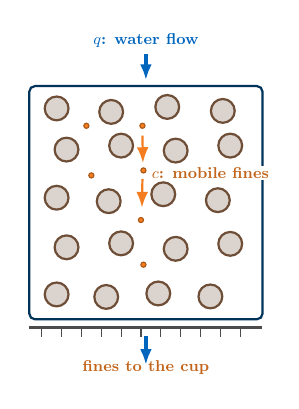
\begin{tikzpicture}[scale=.63,transform shape]
    \draw[rounded corners=2pt,thick,tumdark] (0,0) rectangle (4.7,4.7);
    \draw[arr,line width=1.2pt] (2.35,5.35)--(2.35,4.82);
    \node[tumblue,font=\small\bfseries] at (2.35,5.62) {$q$: water flow};
    \foreach \x/\y in {.55/.5,1.55/.45,2.6/.52,3.65/.46,
      .75/1.45,1.85/1.53,2.95/1.42,4.05/1.52,
      .55/2.45,1.6/2.38,2.7/2.52,3.8/2.4,
      .75/3.42,1.85/3.5,2.95/3.4,4.05/3.5,
      .55/4.25,1.65/4.18,2.78/4.28,3.9/4.2}{\node[grain] at (\x,\y) {};}
    \foreach \x/\y in {1.15/3.9,2.28/3.9,2.3/3.0,1.25/2.9,2.25/2.0,2.3/1.1}
      \node[fine] at (\x,\y) {};
    \draw[arr,tumorange] (2.28,3.7)--(2.29,3.15);
    \draw[arr,tumorange] (2.28,2.83)--(2.27,2.25);
    \node[font=\small\bfseries,tumorange!80!black,fill=white,inner sep=1pt]
      at (3.65,2.95) {$c$: mobile fines};
    \draw[very thick,black!70] (0,-.16)--(4.7,-.16);
    \foreach \x in {.25,.65,...,4.45}{\draw[black!70] (\x,-.16)--(\x,-.36);}
    \draw[arr,line width=1.2pt] (2.35,-.34)--(2.35,-.92);
    \node[font=\small\bfseries,tumorange!80!black] at (2.35,-.98) {fines to the cup};
   \end{tikzpicture}
  \column{0.54\textwidth}
   \small
   \hi{Flow and mobile fines}
   \begin{itemize}
    \item $Q$: flow rate; $A$: puck area; $q=Q/A$: superficial velocity;
    \item $c$: mobile-fines concentration; $q\,c$: advective fines flux.
   \end{itemize}
   \hi{Pore structure and retained fines}
   \begin{itemize}
    \item $\varepsilon$: porosity; $K$: permeability;
    \item $m_{\mathrm a}$: available attached fines; $m_{\mathrm d}$: deposited fines;
    \item $d_f$: fine diameter; $d_h$: local hydraulic diameter.
   \end{itemize}
 \end{columns}
 %\vspace{.2cm}
 %\takeaway{$q\,c$ means $q$ multiplied by $c$; $c$ is not a subscript.}
\end{frame}

% -----------------------------------------------------------------------------
\begin{frame}{The goal is a model that measurements can actually identify}

\vspace*{0.5cm}	
 \question{How can we predict flow, blockage and fines in the cup without hiding the physics inside fitted parameters?}
 \vspace{.35cm}
 \begin{FlexRow}{0.49\textheight}
  \Col{.31}{\centering\hi{CT images}\\[.35em]
   \small Porosity, hydraulic diameter, deposit location and axial heterogeneity}
  \Col{.31}{\centering\hi{Pore networks}\\[.35em]
   \small Permeability, dispersion, particle capture and escape closures}
  \Col{.31}{\centering\hi{Experiments}\\[.35em]
   \small Pressure--flow curves, pump dynamics and time-resolved cup fines}
 \end{FlexRow}
 
 \vspace*{-1cm}
 \takeaway{The equation structure is fixed first; each parameter is assigned to a specific measurement or pore-scale calculation.}
\end{frame}

% -----------------------------------------------------------------------------
\begin{frame}{One-dimensional means ``layers in series''}
 \begin{columns}[T,onlytextwidth]
  \column{.48\textwidth}\centering
   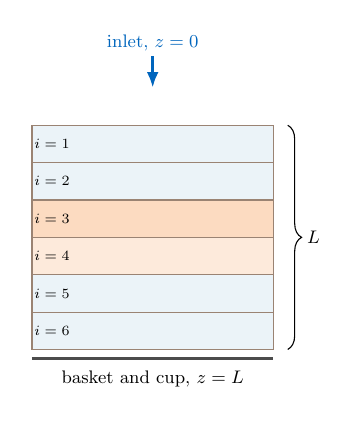
\begin{tikzpicture}[x=1cm,y=1cm,scale=.73,transform shape]
    \draw[arr,line width=1.2pt] (2.1,5.1)--(2.1,4.55);
    \node[tumblue,font=\small] at (2.1,5.34) {inlet, $z=0$};
    \foreach \i/\c in {0/tumlight,1/tumlight,2/tumorange!16,3/tumorange!28,4/tumlight,5/tumlight}{
      \fill[\c] (0,{.65*\i}) rectangle (4.2,{.65*(\i+1)});
      \draw[coffee!70] (0,{.65*\i}) rectangle (4.2,{.65*(\i+1)});
      \node[font=\scriptsize] at (.35,{.65*\i+.325}) {$i=\number\numexpr6-\i\relax$};
    }
    \draw[very thick,black!70] (0,-.16)--(4.2,-.16);
    \node[font=\small] at (2.1,-.52) {basket and cup, $z=L$};
    \draw[decorate,decoration={brace,mirror,amplitude=5pt}] (4.45,0)--(4.45,3.9)
      node[midway,right=6pt,font=\small] {$L$};
   \end{tikzpicture}
  \column{.48\textwidth}\hi{Resolved along the puck height}
   \begin{itemize}\item pressure gradient;
   \item porosity and permeability;
   \item available, mobile and deposited fines.\end{itemize}
   \hi{Not resolved}
   \begin{itemize}\item radial channels;
   \item individual pores or particles;
   \item extraction chemistry.\end{itemize}
 \end{columns}
 \vspace{.25cm}
 \takeaway{The same flow crosses every layer; a blocked layer carries a larger pressure gradient.}
\end{frame}

% -----------------------------------------------------------------------------
\begin{frame}{The model follows fines through five inventories}
 \centering
 
 \vspace*{0.5cm}
 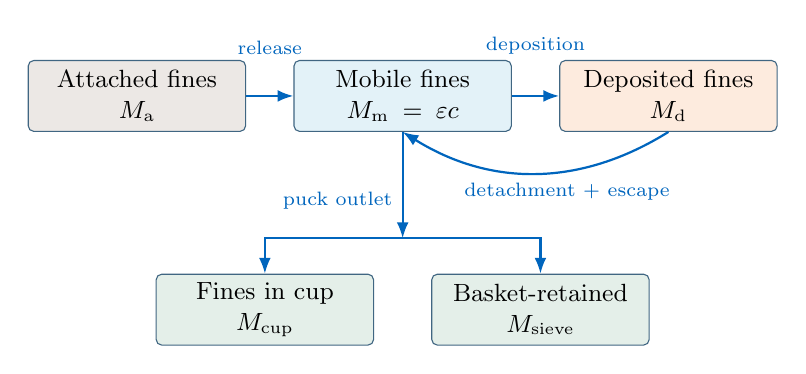
\begin{tikzpicture}[node distance=7mm and 6mm]
  \node[box,fill=coffee!13] (a) {Attached fines\\$M_{\mathrm a}$};
  \node[physicsbox,right=of a] (m) {Mobile fines\\$M_{\mathrm m} =\varepsilon c$};
  \node[box,right=of m,fill=tumorange!15] (d) {Deposited fines\\$M_{\mathrm d}$};
  \node[outputbox,below=18mm of m,xshift=1.75cm] (s) {Basket-retained\\$M_{\mathrm{sieve}}$};
  \node[outputbox,below=18mm of m,xshift=-1.75cm] (cup) {Fines in cup\\$M_{\mathrm{cup}}$};
  \draw[arr] (a)--node[above=4mm,font=\scriptsize]{release}(m);
  \draw[arr] (m)--node[above=4mm,font=\scriptsize]{deposition}(d);
  \draw[arr] (d.south) to[bend left=32] node[below,,xshift=4mm,font=\scriptsize]{detachment + escape} (m.south);
  \coordinate (split) at ($(m.south)+(0,-1.35)$);
  \draw[arr] (m.south)--node[left,yshift=-2mm,font=\scriptsize]{puck outlet}(split);
  \draw[arr] (split)-|(cup.north);
  \draw[arr] (split)-|(s.north);
 \end{tikzpicture}
 \vspace{.65cm}
 \[
 M_0=M_{\mathrm a}+M_{\mathrm m}+M_{\mathrm d}+M_{\mathrm{sieve}}+M_{\mathrm{cup}}.
 \]
 \takeaway{Every fine is accounted for; internal exchange terms cancel in the global mass balance.}
\end{frame}

% -----------------------------------------------------------------------------
\begin{frame}{Three balance equations describe the evolving fines}
 \small
 \begin{align*}
 \frac{\partial(\varepsilon \:c)}{\partial t}
 +\frac{\partial(q\:c)}{\partial z}
 &=\frac{\partial}{\partial z}\!\left(\varepsilon D\frac{\partial c}{\partial z}\right)
 +R_{\mathrm{rel}}-R_{\mathrm{dep}}+R_{\mathrm{wash}},\\[.25em]
 \frac{\partial m_{\mathrm d}}{\partial t}
 &=R_{\mathrm{dep}}-R_{\mathrm{wash}},\\[.25em]
 \frac{\partial m_{\mathrm a}}{\partial t}
 &=-R_{\mathrm{rel}}.
 \end{align*}
 \vspace{.1cm}
 \begin{FlexRow}{0.25\textheight}
  \Col{.31}{\centering\hi{$q\:c$}\\advection carries fines with the water}
  \Col{.31}{\centering\hi{$\varepsilon \: D\,\partial c/\partial z$}\\dispersion spreads the concentration}
  \Col{.31}{\centering\hi{$R$ terms}\\local transfer between inventories}
 \end{FlexRow}
 \takeaway{Only the mobile fines travel between cells; release, deposition and washout are local source terms.}
\end{frame}

% -----------------------------------------------------------------------------
\begin{frame}{Release and deposition describe two opposite transfers}
	\begin{FlexRow}{0.59\textheight}
		
		\Col{.48}{\hi{Release: fines enter the water}
			\[
			R_{\mathrm{rel}}=k_{\mathrm{rel}}\,m_{\mathrm a}
			\left(\frac{|q|}{q_{\mathrm{ref}}}\right)^{a_{\mathrm r}}.
			\]
			\small
			Available fines $m_{\mathrm a}$ are released into the flowing water.
			The release becomes faster with increasing flow; $k_{\mathrm{rel}}$
			sets the timescale and $a_{\mathrm r}$ the flow sensitivity.
			
			\medskip
			Calibrate using fines breakthrough at different flow rates.}
		
		\Col{.48}{\hi{Deposition: mobile fines are captured}
			\[
			R_{\mathrm{dep}}=k_{\mathrm{dep}}\,\chi(z)\,|q|\,c
			\pos{1-\frac{m_{\mathrm d}}{m_{\mathrm{cap}}}}.
			\]
			\small
The transported fines $|q|c$ are captured by the pore structure.
Capture decreases as $m_{\mathrm d}$ approaches the local capacity
$m_{\mathrm{cap}}$. The optional factor $\chi(z)$ represents enhanced
deposition near the basket.
			
			\medskip
			Calibrate using PNM breakthrough and CT deposition profiles.}
	\end{FlexRow}
	
			\vspace*{1cm}
	\takeaway{Release adds fines to the water; deposition stores them in the puck.}
\end{frame}

% -----------------------------------------------------------------------------
\begin{frame}{Washout requires detachment and geometric escape}
	\begin{FlexRow}{0.58\textheight}
		
		\Col{.49}{\hi{Step 1: hydraulic detachment}
			\begin{align*}
				R_{\mathrm{det}}^*
				&=k_{\mathrm{det}}m_{\mathrm d}
				\pos{\frac{G}{G_{\mathrm{crit}}}-1}^{b},\\[-.2em]
				G&=\left|\frac{\partial p}{\partial z}\right|.
			\end{align*}
			\small
			Deposits detach only when the pressure gradient exceeds
			$G_{\mathrm{crit}}$. Above this threshold, stronger loading produces
			faster detachment.
			
			\medskip
			Calibrate using pressure-pulse experiments.}
		
		\Col{.47}{\hi{Step 2: geometric escape}
			\[
			\lambda=\frac{d_f}{d_h},\qquad
			R_{\mathrm{wash}}=P_{\mathrm{esc}}(\lambda)R_{\mathrm{det}}^*,
			\]
			\[
			P_{\mathrm{esc}}
			=\frac{1}{1+\exp[s(\lambda-\lambda_c)]}.
			\]
			\small
			A detached fine escapes only if it is small enough relative to the
			available pore size: small $\lambda$ means easier escape.
			
			\medskip
			CT provides $d_h$, the PSD provides $d_f$, and PNM calibrates
			$P_{\mathrm{esc}}$.}
		
	\end{FlexRow}
	
	\vspace*{1cm}
	\takeaway{Detachment breaks adhesion; geometric escape determines actual washout.}
\end{frame}

% -----------------------------------------------------------------------------
\begin{frame}{The PSD is reduced to quantities used by the 1D closures}
 \begin{FlexRow}{0.60\textheight}
  \Col{.45}{\hi{Measured bimodal PSD}
   \begin{itemize}\item Fit a five-parameter mixture model.
   \item Choose a mobility cutoff $d_{\mathrm{cut}}$.
   \item Integrate the fine fraction below the cutoff.
   \item Calculate representative fine and coarse diameters.\end{itemize}}
  \Col{.51}{\centering
   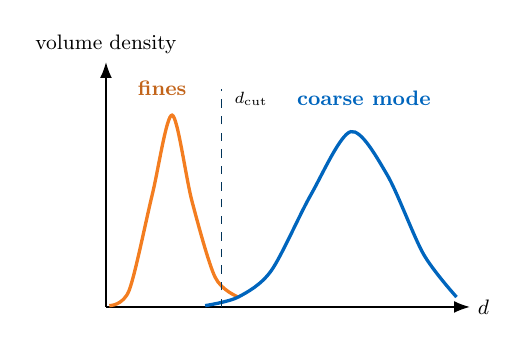
\begin{tikzpicture}[x=1cm,y=1cm,scale=.84,transform shape]
    \draw[-{Latex[length=2mm]}] (0,0)--(5.5,0) node[right,font=\small] {$d$};
    \draw[-{Latex[length=2mm]}] (0,0)--(0,3.7) node[above,font=\small] {volume density};
    \draw[tumorange,very thick,smooth] plot coordinates{(.05,.02)(.35,.25)(.7,1.7)(1.0,2.9)(1.3,1.6)(1.65,.45)(2.0,.15)};
    \draw[tumblue,very thick,smooth] plot coordinates{(1.5,.02)(2.0,.15)(2.5,.55)(3.1,1.7)(3.7,2.65)(4.25,2.0)(4.8,.8)(5.3,.15)};
    \draw[dashed,tumdark] (1.75,0)--(1.75,3.3);
    \node[font=\scriptsize,anchor=west] at (1.82,3.15) {$d_{\mathrm{cut}}$};
    \node[tumorange!80!black,font=\small\bfseries] at (.85,3.3) {fines};
    \node[tumblue,font=\small\bfseries] at (3.9,3.15) {coarse mode};
   \end{tikzpicture}}
 \end{FlexRow}
 \begin{center}\small
  $f_{\mathrm{fine}}\rightarrow m_{\mathrm a,0}$, \quad
  $d_f\rightarrow d_f/d_h$, \quad
  $d_{\mathrm{eff}}\rightarrow d_{h,0}$ and Ergun baseline.
 \end{center}
 \slidesource{Source: Bora and Briesen, Journal of Food Process Engineering 49 (2026), e70645.}
\end{frame}

% -----------------------------------------------------------------------------
\begin{frame}{Deposits change porosity and permeability}
 \begin{FlexRow}{0.58\textheight}
  \Col{.44}{\hi{Porosity decreases}
   \[
    \varepsilon=\max\!\left(\varepsilon_0-\frac{m_{\mathrm d}}{\rho_{\mathrm d}},\,\varepsilon_{\min}\right).
   \]
   \hi{Permeability controls resistance}
   \[
    \frac{K}{K_0}=\exp\!\left(-\beta\frac{m_{\mathrm d}}{m_{\mathrm{cap}}}\right)
   \]
   \small with a configured lower bound.}
  \Col{.52}{\hi{Three selectable closures}
   \begin{itemize}\item exponential deposit law;
   \item Kozeny--Carman-style porosity law;
   \item tabulated $m_{\mathrm d}\mapsto K/K_0$ from PNM.\end{itemize}
   \vspace{.25cm}
   \small The PNM table is preferred when reconstructed pore networks are available: it preserves the simulated relation rather than forcing it into one empirical equation.}
 \end{FlexRow}
 
 \vspace*{0.5cm}
 \takeaway{CT and PNM determine the initial structure; repeated PNM calculations determine how blockage changes conductance.}
\end{frame}

% -----------------------------------------------------------------------------
\begin{frame}{Darcy--Forchheimer converts structure into pressure loss}
 \question{What pressure gradient is needed to drive the common superficial velocity $q=Q/A$?}
 \vspace{.35cm}
 \[
  G(z,t)=\underbrace{\frac{\mu q}{K(z,t)}}_{\text{viscous Darcy term}}
  +\underbrace{\rho\beta_F(z,t)|q|q}_{\text{nonlinear inertial term}}.
 \]
 \vspace{.2cm}
 \[
  \Delta p_{\mathrm{puck}}
  =q\int_0^L\frac{\mu}{K}\,\mathrm dz
  +q^2\int_0^L\rho\beta_F\,\mathrm dz \qquad (q\ge0).
 \]
 \begin{center}\small
 $K$: permeability from CT--PNM or low-flow measurements; \quad
 $\beta_F$: Forchheimer coefficient from PNM or curvature in $\Delta p(Q)$.
 \end{center}
 \takeaway{The model does not solve a momentum PDE; it evaluates and integrates this local resistance law.}
\end{frame}

% -----------------------------------------------------------------------------
\begin{frame}{Why not use the Ergun equation directly?}
 \begin{columns}[T,onlytextwidth]
  \column{.31\textwidth}\centering\hi{Darcy only}\\[.35em]
   \small Uses structural permeability $K$, but assumes pressure loss is linear in flow.\\[.45em]
   \color{tumgray}Best for sufficiently slow flow.
  \column{.34\textwidth}\centering\hi{Direct Ergun}\\[.35em]
   \small Predicts both terms from porosity, sphericity and one effective diameter.\\[.45em]
   \color{tumgray}Useful baseline, but compresses connectivity and bottlenecks into bulk descriptors.
  \column{.31\textwidth}\centering\hi{Darcy--Forchheimer}\\[.35em]
   \small Keeps CT--PNM $K$ and adds a separately calibratable inertial coefficient $\beta_F$.\\[.45em]
   \color{tumred}Selected formulation.
 \end{columns}
 \vspace{.45cm}
 \[
 \beta_{F,\mathrm{Ergun}}=\frac{1.75(1-\varepsilon)}{\varepsilon^3d_{\mathrm{eff}}}
 \quad\text{provides an initial comparison, not a mandatory closure.}
 \]
 \takeaway{We retain Ergun's nonlinear physics without discarding the permeability resolved from the real pore structure.}
\end{frame}

% -----------------------------------------------------------------------------
\begin{frame}{The basket and machine are separate from the coffee puck}
 \begin{FlexRow}{0.61\textheight}
  \Col{.48}{\hi{Simple basket model}
   \begin{align*}
    \Delta p_{\mathrm{total}}&=\Delta p_{\mathrm{puck}}+Q R_s,\\
    \dot M_{\mathrm{cup}}&=(1-\eta_s)\dot M_{\mathrm{out,puck}},\\
    \dot M_{\mathrm{sieve}}&=\eta_s\dot M_{\mathrm{out,puck}}.
   \end{align*}
   \small $R_s$ and $\eta_s$ are constant. Basket deposits do not yet alter resistance.}
  \Col{.48}{\hi{PI-controlled pump}
   \begin{align*}
    e&=p_{\mathrm{set}}-p,\\
    Q_{\mathrm{raw}}&=Q_{\mathrm{ff}}+K_Pe+K_I\!\int e\,dt,\\
    Q_{\mathrm{cmd}}&=\operatorname{clip}(Q_{\mathrm{raw}},0,Q_{\max}).
   \end{align*}
   \small Pump lag and anti-windup are included. A coarse permeable puck can remain below 9 bar when $Q_{\max}$ is reached.}
 \end{FlexRow}
 \takeaway{Empty-basket tests characterize $R_s$ and the machine before any puck kinetics are fitted.}
\end{frame}

% -----------------------------------------------------------------------------
\begin{frame}{Initial and boundary conditions complete the mathematical problem}
 \begin{FlexRow}{0.59\textheight}
  \Col{.48}{\hi{At $t=0$}
   \begin{itemize}\item $m_{\mathrm a}=m_{\mathrm a,0}$;
   \item $m_{\mathrm d}=m_{\mathrm d,0}$;
   \item $c=c_0$;
   \item $\varepsilon_0(z)$ and $K_0(z)$ are uniform or supplied as CT--PNM profiles.\end{itemize}}
  \Col{.48}{\hi{At the boundaries}
   \begin{itemize}\item clean water enters: $(q\:c)_{z=0}=0$;
   \item zero dispersive flux at $z=0,L$;
   \item mobile fines leave convectively: $\dot M_{\mathrm{out}}=A\,q\,c(L,t)$;
   \item cup pressure is the zero-gauge reference.\end{itemize}}
 \end{FlexRow}
 \takeaway{Reverse flow and radial bypass channels are outside the present 1D model.}
\end{frame}

% -----------------------------------------------------------------------------
\begin{frame}{The finite-volume method enforces flux balance cell by cell}
 \centering
 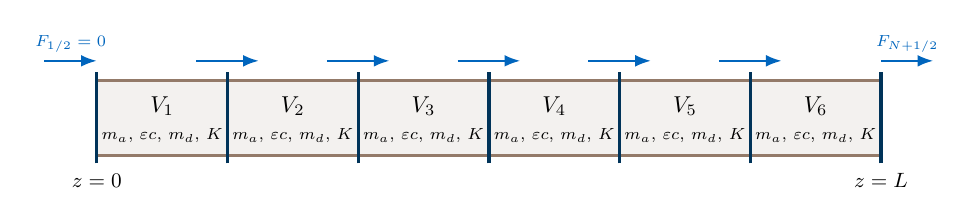
\begin{tikzpicture}[x=1cm,y=1cm,scale=.83,transform shape,
  cell/.style={fill=coffee!8,draw=coffee!75,thick},
  face/.style={very thick,tumdark},
  flux/.style={-{Latex[length=2mm]},thick,tumblue}]
  \draw[flux] (-.8,1.45)--(0,1.45) node[midway,above,font=\scriptsize] {$F_{1/2}=0$};
  \foreach \i [evaluate=\i as \x using 2*(\i-1)] in {1,...,6}{
    \draw[cell] (\x,0) rectangle ({\x+2},1.15);
    \node at ({\x+1},.76) {$V_{\i}$};
    \node[font=\scriptsize] at ({\x+1},.30) {$m_a,\,\varepsilon c,\,m_d,\,K$};}
  \foreach \x in {0,2,4,6,8,10,12}{\draw[face] (\x,-.12)--(\x,1.28);}
  \foreach \x in {2,4,6,8,10}{\draw[flux] ({\x-.48},1.45)--({\x+.48},1.45);}
  \draw[flux] (12,1.45)--(12.8,1.45) node[midway,above,font=\scriptsize] {$F_{N+1/2}$};
  \node[font=\small] at (0,-.38) {$z=0$};
  \node[font=\small] at (12,-.38) {$z=L$};
 \end{tikzpicture}
 \vspace{.15cm}

\[
\frac{(\varepsilon c)_i^{n+1}-(\varepsilon c)_i^n}{\Delta t}
=
-\frac{F_{i+1/2}-F_{i-1/2}}{\Delta z}
+R_{\mathrm{rel},i}-R_{\mathrm{dep},i}+R_{\mathrm{wash},i}.
\]

\[
F_{i+1/2}
=
\underbrace{q\,c_i}_{\text{advection}}
-
\underbrace{
	\varepsilon_{i+1/2}D
	\frac{c_{i+1}-c_i}{\Delta z}
}_{\text{dispersion}},
\qquad q\geq 0.
\]

\small
$F_{i+1/2}$ is the total fines-mass flux through the face between
cells $i$ and $i+1$.
Upwind advection uses the concentration in the upstream cell, while
centred dispersion uses the concentration difference between both cells.
\end{frame}

% -----------------------------------------------------------------------------
\begin{frame}{Velocity and pressure are calculated algebraically}
	\begin{columns}[T,onlytextwidth]
		
		\column{0.47\textwidth}
		\hi{One common superficial velocity}
		\[
		\frac{\partial q}{\partial z}=0
		\qquad\Longrightarrow\qquad
		q(t)=\frac{Q(t)}{A}.
		\]
		
		\small
		The flow rate is determined by the selected operating mode:
		
		\begin{itemize}
			\item prescribed directly in flow mode;
			\item obtained from the pressure condition in pressure mode;
			\item determined by the pump and PI controller in PI mode.
		\end{itemize}
		
		The local pore velocity is then
		
		\[
		u_{\mathrm{pore},i}=\frac{q}{\varepsilon_i}.
		\]
		
		\column{0.49\textwidth}
		\hi{Pressure is reconstructed cell by cell}
		
		\[
		G_i=
		\frac{\mu q}{K_i}
		+\rho\beta_{F,i}|q|q,
		\]		
		\[
		\Delta p_i=G_i\Delta z.
		\]
		
		Starting from the pressure above the basket,		
		\[
		p_{N+1/2}=Q R_s,
		\]
		
		the pressure is accumulated towards the inlet:		
		\[
		p_{i-1/2}
		=
		p_{i+1/2}+G_i\Delta z.
		\]
		
		\small
		A cell with lower permeability therefore produces a larger
		local pressure drop.
		
	\end{columns}
	
	\vspace{0.25cm}
	\takeaway{The fines concentration is solved by FVM; velocity and pressure
		are obtained from continuity and the Darcy--Forchheimer resistance.}
\end{frame}

% -----------------------------------------------------------------------------
\begin{frame}{Each time step closes a feedback loop}
 \centering
 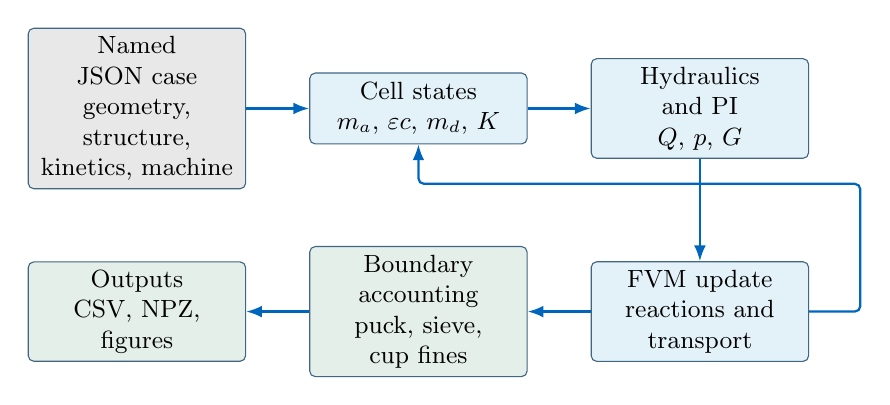
\begin{tikzpicture}[node distance=5mm and 8mm]
  \node[databox] (inputs) {Named JSON case\\geometry, structure, kinetics, machine};
  \node[physicsbox,right=of inputs] (state) {Cell states\\$m_a$, $\varepsilon c$, $m_d$, $K$};
  \node[physicsbox,right=of state] (hyd) {Hydraulics and PI\\$Q$, $p$, $G$};
  \node[physicsbox,below=13mm of hyd] (update) {FVM update\\reactions and transport};
  \node[outputbox,left=of update] (basket) {Boundary accounting\\puck, sieve, cup fines};
  \node[outputbox,left=of basket] (outputs) {Outputs\\CSV, NPZ, figures};
  \draw[arr] (inputs)--(state); \draw[arr] (state)--(hyd);
  \draw[arr] (hyd)--(update); \draw[arr] (update)--(basket);
  \draw[arr] (basket)--(outputs);
  \draw[arr,rounded corners=2pt] (update.east)--++(.65,0)
    |- ([yshift=-5mm]state.south)--(state.south);
 \end{tikzpicture}
 \vspace{.35cm}
 \par\vspace{.45cm}
 \small\centering Deposit changes $\varepsilon$, $K$ and $d_h$; these change pressure and flow; the new hydraulics then alter release, deposition and washout.
 \takeaway{The coupling is dynamic even though the hydraulic relation itself is algebraic.}
\end{frame}

% -----------------------------------------------------------------------------
\begin{frame}{Calibration starts with structure and hydraulics}
 \scriptsize
 \begin{tabular}{>{\raggedright\arraybackslash}p{2.45cm} >{\raggedright\arraybackslash}p{4.05cm} >{\raggedright\arraybackslash}p{5.55cm}}
  \toprule
  \textbf{Category} & \textbf{Model inputs} & \textbf{How they are obtained}\\
  \midrule
  Measured and fixed & $L$, $A$, $\mu$, $\rho$, dose, five PSD parameters & Geometry and temperature measurements; laser-diffraction PSD fit; calculate fines fraction and representative diameters.\\[.35em]
  CT-derived structure & $\varepsilon_0(z)$, $d_{h,0}(z)$, deposit location & Segment axial slabs; calculate connected porosity and $d_h=4V_{\mathrm{void}}/A_{\mathrm{wetted}}$; quantify segmentation uncertainty.\\[.35em]
  PNM-derived closures & $K_0(z)$, $D$, $K/K_0(m_d)$, capture, $P_{\mathrm{esc}}(d_f/d_h)$ & Solve flow and particle transport on CT-derived networks; export depth profiles and lookup tables.\\[.35em]
  Hydraulic experiments & global $K$ scale, $\beta_F$, clean-basket $R_s$ & Fit $\Delta p=c_1Q+c_2Q^2$ over several flows; low-flow slope constrains $K$, curvature constrains $\beta_F$.\\
  \bottomrule
 \end{tabular}
 \vfill
 \takeaway{These quantities should be fixed before fitting fines-release or detachment kinetics.}
\end{frame}

% -----------------------------------------------------------------------------
\begin{frame}{Dynamic experiments identify the remaining rates}
 \begin{FlexRow}{0.59\textheight}
  \Col{.47}{\hi{Machine characterization}
   \begin{itemize}\item free-flow and loaded pump curves;
   \item pump time constant $\tau_p$;
   \item flow cap $Q_{\max}$;
   \item PI gains and pressure target.\end{itemize}
   \small Fix these using known hydraulic resistances.}
  \Col{.49}{\hi{Fines dynamics}
   \begin{itemize}\item early cup-fines curve $\rightarrow$ release;
   \item outlet PSD $\rightarrow$ size selectivity;
   \item interrupted CT/PNM $\rightarrow$ deposition location;
   \item pressure pulses $\rightarrow G_{\mathrm{crit}}, k_{\mathrm{det}}$;
   \item basket mass $\rightarrow\eta_s$.\end{itemize}}
 \end{FlexRow}
 \takeaway{Use multiple data types and validate on withheld pucks or grinding levels; do not fit every parameter to one pressure curve.}
\end{frame}

% -----------------------------------------------------------------------------
\begin{frame}{The illustrative case develops strong viscous blockage}
 \begin{FlexRow}{0.67\textheight}
  \Col{.66}{\centering\safeimage{hydraulic_response.png}{\linewidth}{5.25cm}}
  \Col{.30}{\small
   \hi{At 60 s}
   \begin{itemize}\item total pressure: 8.99 bar;
   \item flow: 0.045 mL/s;
   \item minimum $K/K_0$: 0.0126.\end{itemize}
   \vspace{.25cm}
   \hi{Interpretation}

   The PI controller approaches 9 bar while the increasing puck resistance strongly reduces flow.}
 \end{FlexRow}
 \slidesource{Generated by the current Python solver; parameters are illustrative and not experimentally calibrated.}
\end{frame}

% -----------------------------------------------------------------------------
\begin{frame}{The model distinguishes puck washout from fines in the cup}
 \begin{FlexRow}{0.67\textheight}
  \Col{.61}{\centering\safeimage{fines_washout.png}{\linewidth}{5.25cm}}
  \Col{.35}{\small
   \hi{Cumulative masses}
   \begin{itemize}\item puck outlet: 0.0614 g;
   \item basket retained: 0.0215 g;
   \item cup: 0.0399 g.\end{itemize}
   \vspace{.25cm}
   With $\eta_s=0.35$, the basket retains 35\% of the fines that leave the puck.}
 \end{FlexRow}
 \slidesource{Generated by the current Python solver; level-1 basket retention is constant.}
\end{frame}

% -----------------------------------------------------------------------------
\begin{frame}{The axial fields locate the effective blocking region}
 \begin{FlexRow}{0.67\textheight}
  \Col{.49}{\centering\safeimage{deposited_fines.png}{\linewidth}{5.25cm}}
  \Col{.49}{\centering\safeimage{relative_permeability.png}{\linewidth}{5.25cm}}
 \end{FlexRow}
 \vspace{.1cm}
 \takeaway{These fields can be compared with interrupted CT reconstructions, but a 1D layer cannot represent lateral channel geometry.}
 \slidesource{Generated by the current Python solver; parameters are illustrative.}
\end{frame}

% -----------------------------------------------------------------------------
\begin{frame}{Verification and validation answer different questions}
 \begin{FlexRow}{0.61\textheight}
  \Col{.47}{\hi{Verification: is the code correct?}
   \begin{itemize}\item exact Darcy and Darcy--Forchheimer solutions;
   \item exact pressure-to-flow inversion;
   \item conservation and positivity;
   \item non-oscillatory pure advection;
   \item grid and timestep refinement;
   \item PI and pump-cap limits.\end{itemize}}
  \Col{.49}{\hi{Validation: is the model physically adequate?}
   \begin{itemize}\item measured pressure and flow;
   \item CT-derived axial structural changes;
   \item PNM permeability and particle transport;
   \item cup-fines mass and outlet PSD;
   \item withheld grind settings or pucks.\end{itemize}}
 \end{FlexRow}
 \takeaway{Current status: 15/15 unit tests and 17/17 extended verification checks pass; physical validation remains the next stage.}
\end{frame}

% -----------------------------------------------------------------------------
\begin{frame}{The next experiments make the model predictive}
 \centering
 
 \vspace*{0.5cm}
 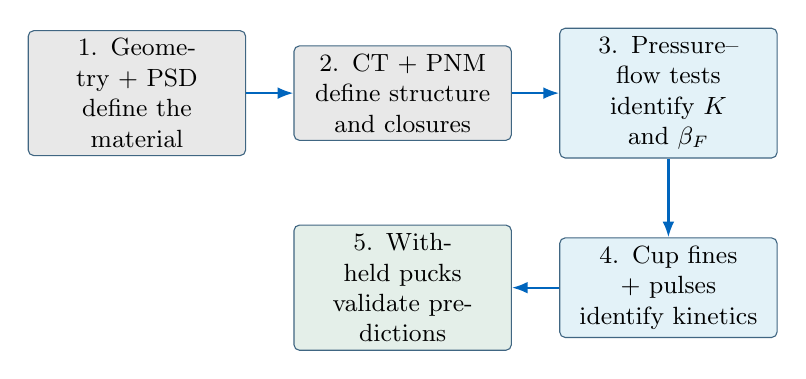
\begin{tikzpicture}[node distance=6mm and 6mm]
  \node[databox] (psd) {1. Geometry + PSD\\define the material};
  \node[databox,right=of psd] (ct) {2. CT + PNM\\define structure and closures};
  \node[physicsbox,right=of ct] (hyd) {3. Pressure--flow tests\\identify $K$ and $\beta_F$};
  \node[physicsbox,below=10mm of hyd] (kin) {4. Cup fines + pulses\\identify kinetics};
  \node[outputbox,left=of kin] (val) {5. Withheld pucks\\validate predictions};
  \draw[arr] (psd)--(ct); \draw[arr] (ct)--(hyd);
  \draw[arr] (hyd)--(kin); \draw[arr] (kin)--(val);
 \end{tikzpicture}
 \vspace{.30cm}
 \question{A transparent 1D model becomes valuable when every closure is tied to an observable experiment or a pore-network calculation.}
 
 \vspace{-0.2cm}
 \small\centering Immediate software extension: derive the fines fraction and representative diameters directly from the five PSD parameters.
\end{frame}

% -----------------------------------------------------------------------------
\begin{frame}{References and model documentation}
 \small
 \begin{itemize}
  \item M. Bora and H. Briesen, ``Characterization of Bimodal Particle Size Distribution of Ground Coffee Powder,'' \emph{Journal of Food Process Engineering}, 49, e70645, 2026. \texttt{doi:10.1111/jfpe.70645}
  \item S. Ergun, ``Fluid Flow through Packed Columns,'' \emph{Chemical Engineering Progress}, 48, 89--94, 1952.
  \item FineFlow--Espresso technical report, Python solver, named-case configuration and automated verification suite accompanying this presentation.
 \end{itemize}
 %\vspace{.55cm}
% \takeaway{All numerical plots in this presentation were generated by the supplied Python package.}
\end{frame}

\end{document}
